%% 
%% Copyright 2016 Icm Ltd
\documentclass[final,3p]{CSP}

%%%%% PACKAGES %%%%%
\usepackage{amssymb}
\usepackage{changepage}
\usepackage{enumitem}
\usepackage{graphicx}
\usepackage{subcaption}
\usepackage{float}
\usepackage{hyperref}
\usepackage{cleveref}

\hypersetup{
	colorlinks=true,
	linkcolor=blue,
	filecolor=magenta,      
	urlcolor=cyan,
}

%%%%% OPTIONS %%%%%
\biboptions{round,sort,comma,authoryear}
\setlength{\parskip}{5pt}
\setlength\parindent{0pt}

\captionsetup[subfigure]{labelformat=parens, labelsep = space} 


\def \FigPath {./figures} 

%%%%% PAPER %%%%%
\begin{document}
	
	%Article Type: \textbf{Technical}\\
	Word Count: \textbf{TBD}\\
	Submitted: \textbf{May 22nd, 2020}
	
	\begin{frontmatter}
		
		\title{Classifying the Stability of 2D Block Assemblies using a Convolutional Neural Network}
		
		\author{Edvard P.G. Bruun\corref{cor}}
		\ead{ebruun@princeton.edu}
		
		\cortext[cor]{Corresponding author}
		
		\begin{keyword}\rm
			\begin{adjustwidth}{2cm}{2cm}{\itshape\textbf{Keywords:}}
				word1, word2, word3
			\end{adjustwidth}
		\end{keyword}
		
		\begin{abstract}\rm
			\begin{adjustwidth}{2cm}{2cm}{\itshape\textbf{Abstract:}} 
				Summary...
			\end{adjustwidth}
		\end{abstract}
	\end{frontmatter}
	
	RESEARCH HIGHLIGHTS:
	\begin{enumerate}
		\item ...
		\item ...
		\item ...
	\end{enumerate}

	
	\clearpage
	\setcounter{page}{1}
	\newpage
	%%%%%%%%%%%%%%%%%%%%%%%%%%%%
	\section{Introduction}
		This is the final paper for the ARC737 reading course (based on the ARC374: Computational Design). The goal for this assignment was to take one of the topics explored in the course and develop it further through an independent study. The topic of Machine Learning (ML) was selected. 
		
		This paper seeks to explore whether  a machine learning algorithm, specifically a Convolutional Neural Net (CNN), can be used to make accurate predictions about some characteristic of a structural system. This is a fairly broad question, so to narrow it down to fit within the confines of the course, the specific goal was to use a CNN to classify the stability of planar discrete element assemblies (i.e. towers built from blocks). This topic was selected for its potential relevance to robotic fabrication, where the assembly of discrete elements is a common construction approach. This work will hopefully act as the beginning of an algorithmic design process that can eventually be coupled with robotic fabrication methods. 
		
		This project is divided into three equal parts:
		\begin{enumerate}
			\item Creating the training set (\Cref{sec:dataset})
			\item Creating the neural network 
			\item Testing and evaluating results
		\end{enumerate}
		
	\section{Conceptual Overview}
	
		Machine learning, in all its various forms, is applicable to a wide variety of tasks, from traditional image classification to natural language processing. But regardless of the specific task, all machine learning applications share the fundamental requirement of needing data from which they can construct a mathematical model. A typical ML workflow can be split up into two distinct phases: training the model, and testing the trained model.
		
		Throughout the training process, the weights of the variables that define the model (e.g. a deep neural net) are adjusted so that the error is minimized over all the avaiable data. Once a sufficient level of accuracy is achieved, this model is deemed ready to be used to make predictions about new data. The level of accuracy that is achieved by the model is based on the quantity and quality of the data, and the robustness of the machine learning framework being used (i.e. deep or shallow, number of hidden layers, number of convolutional layers etc.). In theory, if a proper dataset and framework are used, the model should be able to learn the various features that define the problem (e.g. classifiying a handwritten digit, identifying a type of animal etc.), which then allows it to correctly label any new data.
		
		As data is the most important element of a machine learning model, researchers working on the computational aspects of ML will often use common validated datasets as their benchmarks. In the case of this project, the goal is not just on developing an adequate CNN, but also to have it be applicable to the chosen problem of structural stability. As such, since there is no pre-existing image dataset for the classification of discrete element stability, creating this dataset was a major part of the project.
		 
		 
	\section{Creating the Training and Test Datasets}\label{sec:dataset}
	
		The final dataset consisted of 35,000 images (training = 30,000, testing = 5,000) of unique quadrilateral assemblies  (both rectangular and freeform blocks). The images are tagged with either the ``stable'' or ``unstable'' label (\Cref{fig:dist}) based on the the results of a structural analysis. The data was generated in a random process that resulted in an uneven distribution across the two labels, but since the training set was large  this skew did not seem to adversely affect results. These datasets can be accessed at the following link: (provide github link).
		
		\newpage
		\begin{figure}[h]
			\centering
			%
			\begin{subfigure}[b]{0.44\textwidth}
				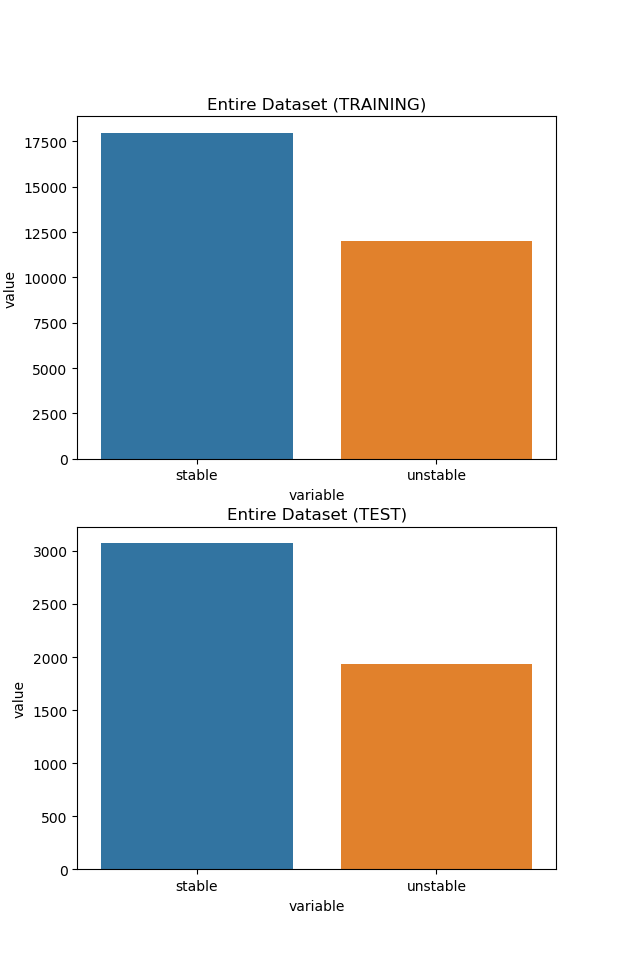
\includegraphics [trim={0.5cm 12.5cm 0cm 2.9cm},clip,width=1\textwidth]{\FigPath/dist}
				\caption{Training Set (Total: 30k)}
				\label{fig:dist_train}
			\end{subfigure}
			%
			\begin{subfigure}[b]{0.44\textwidth}
				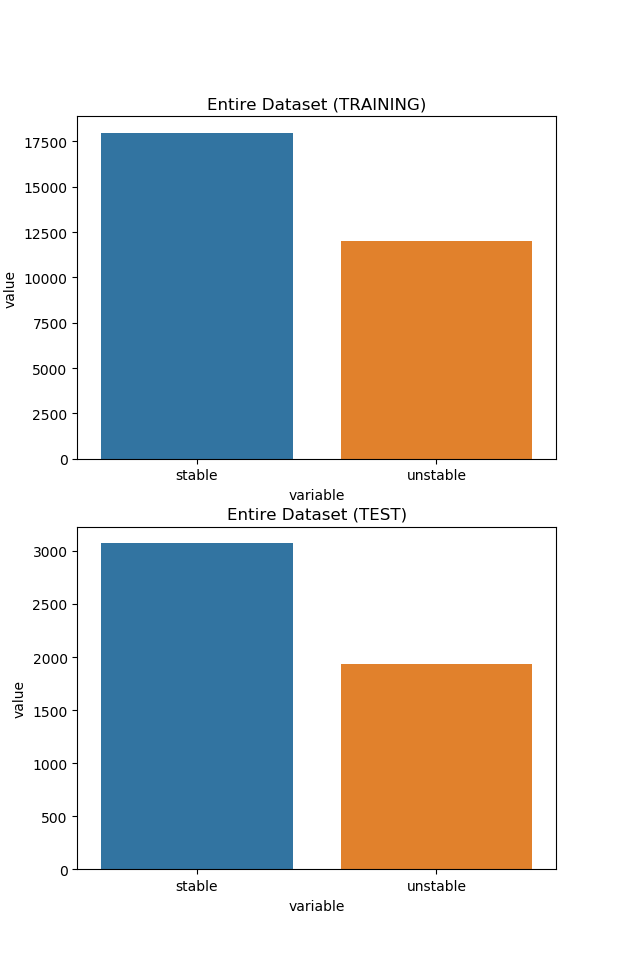
\includegraphics [trim={0.6cm 2.1cm 0cm 13.4cm},clip,width=1\textwidth]{\FigPath/dist}
				\caption{Test Set (Total: 5k)}
				\label{fig:dist_test}
			\end{subfigure}
			%
			\caption{Distribution of labels in Datasets}
			\label{fig:dist}
		\end{figure} 
		
		This dataset was created mainly through the Rhino/Grasshopper interface, although the structural analysis procedure was run outside this environment through a separate script. Grasshopper was chosen as the main platform due to its ability to parametrically script, create and visualize complex 3D objects. While the generated images are just planar representations, the actual tower is modelled as a stack of  3D blocks made from surfaces (\Cref{fig:towers}). The resulting action on the structure is 2D since the blocks are uniformly extruded in the third dimension. The fact that 3D geometry is already modelled and passed to the structural analysis module means that the whole process can easily be extended to assemblies with out-of-plane effects.
		
		\begin{figure}[h]
			\centering
			%
			\begin{subfigure}[b]{0.6\textwidth}
				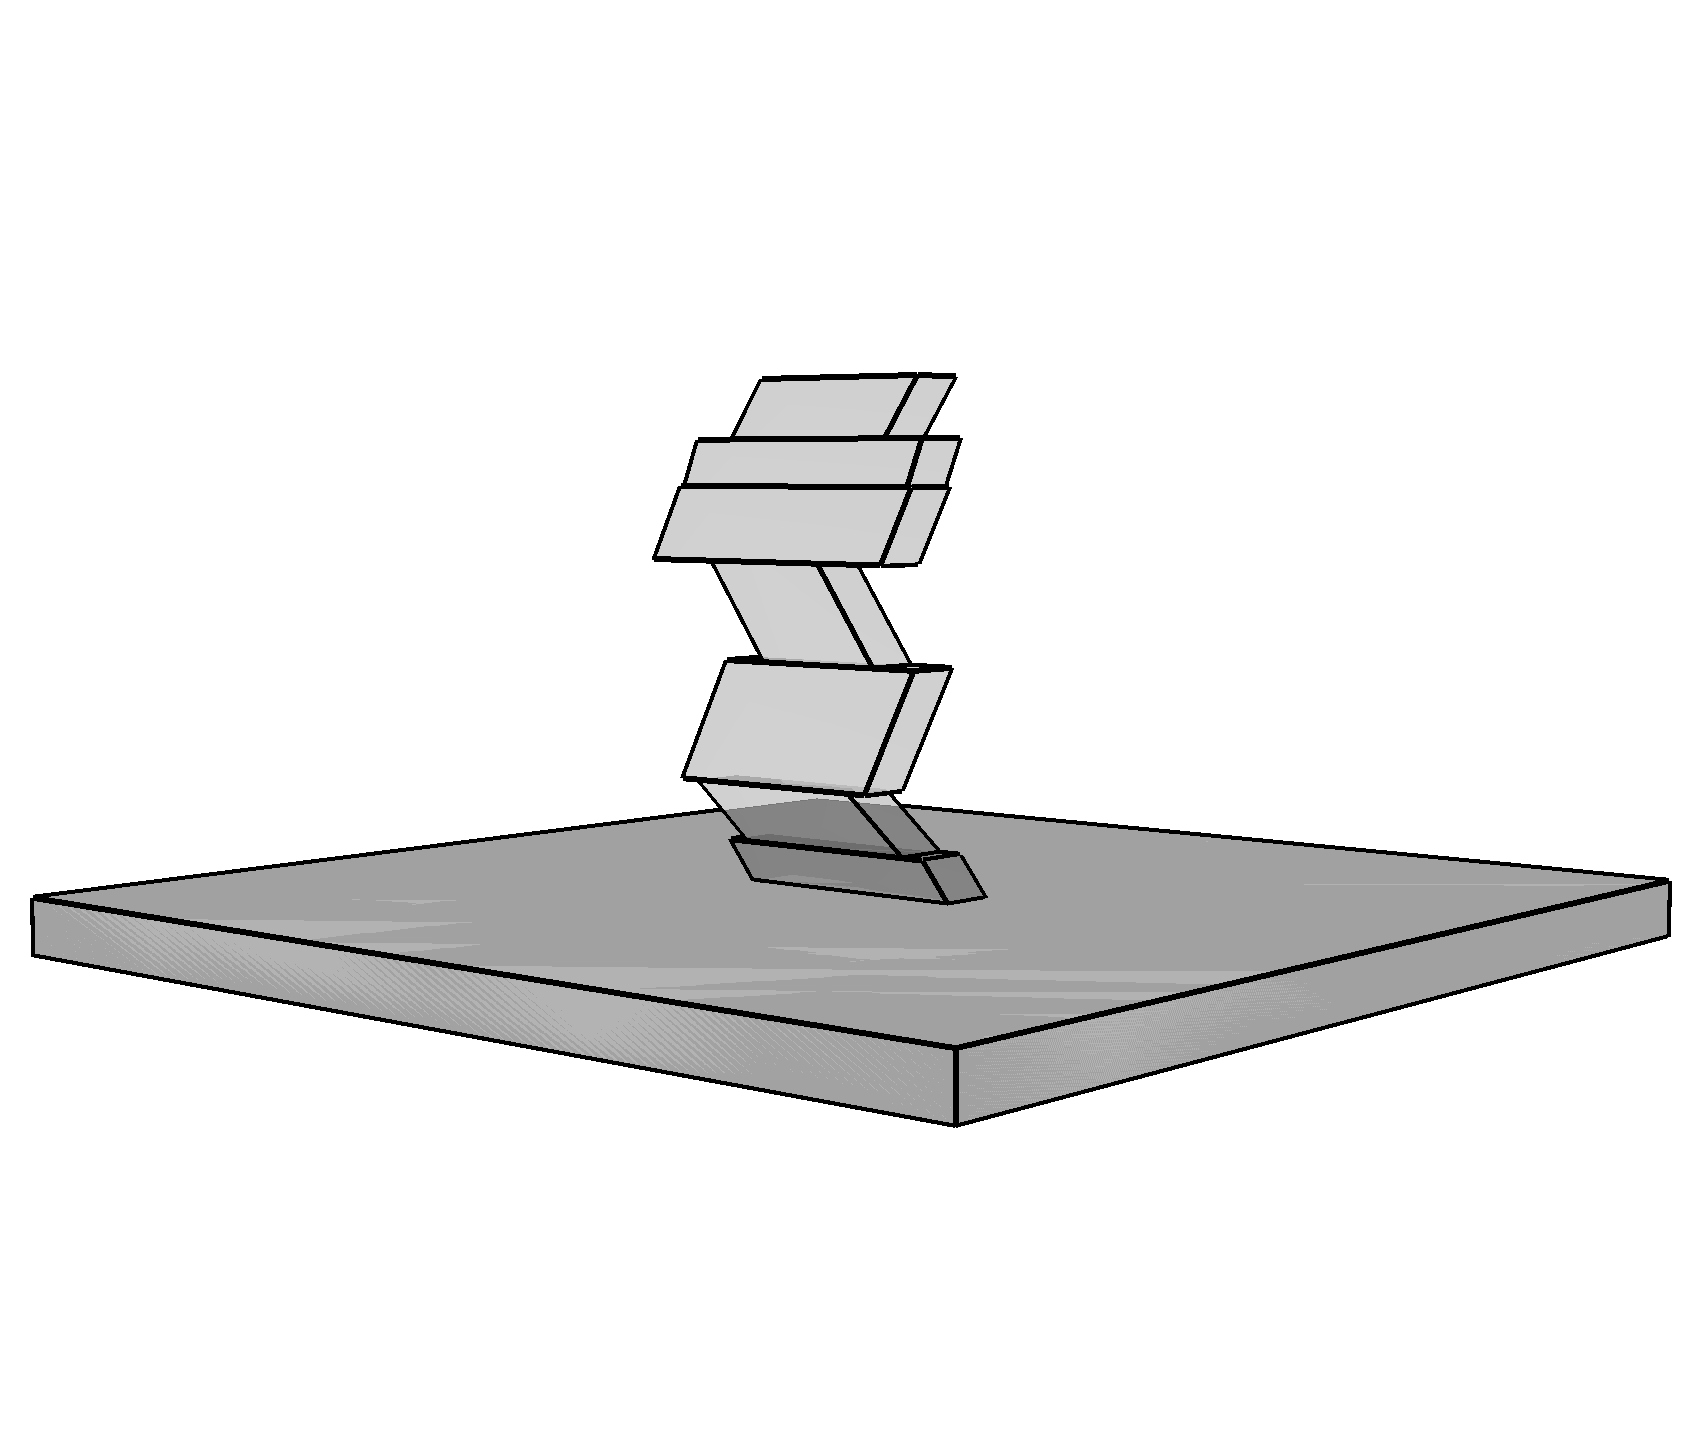
\includegraphics [trim={0.0cm 3cm 0cm 0.0cm},clip,width=1\textwidth]{\FigPath/tower3d}
				\caption{3D Tower}
				\label{fig:t_3d}
			\end{subfigure}
			%
			\begin{subfigure}[b]{0.39\textwidth}
				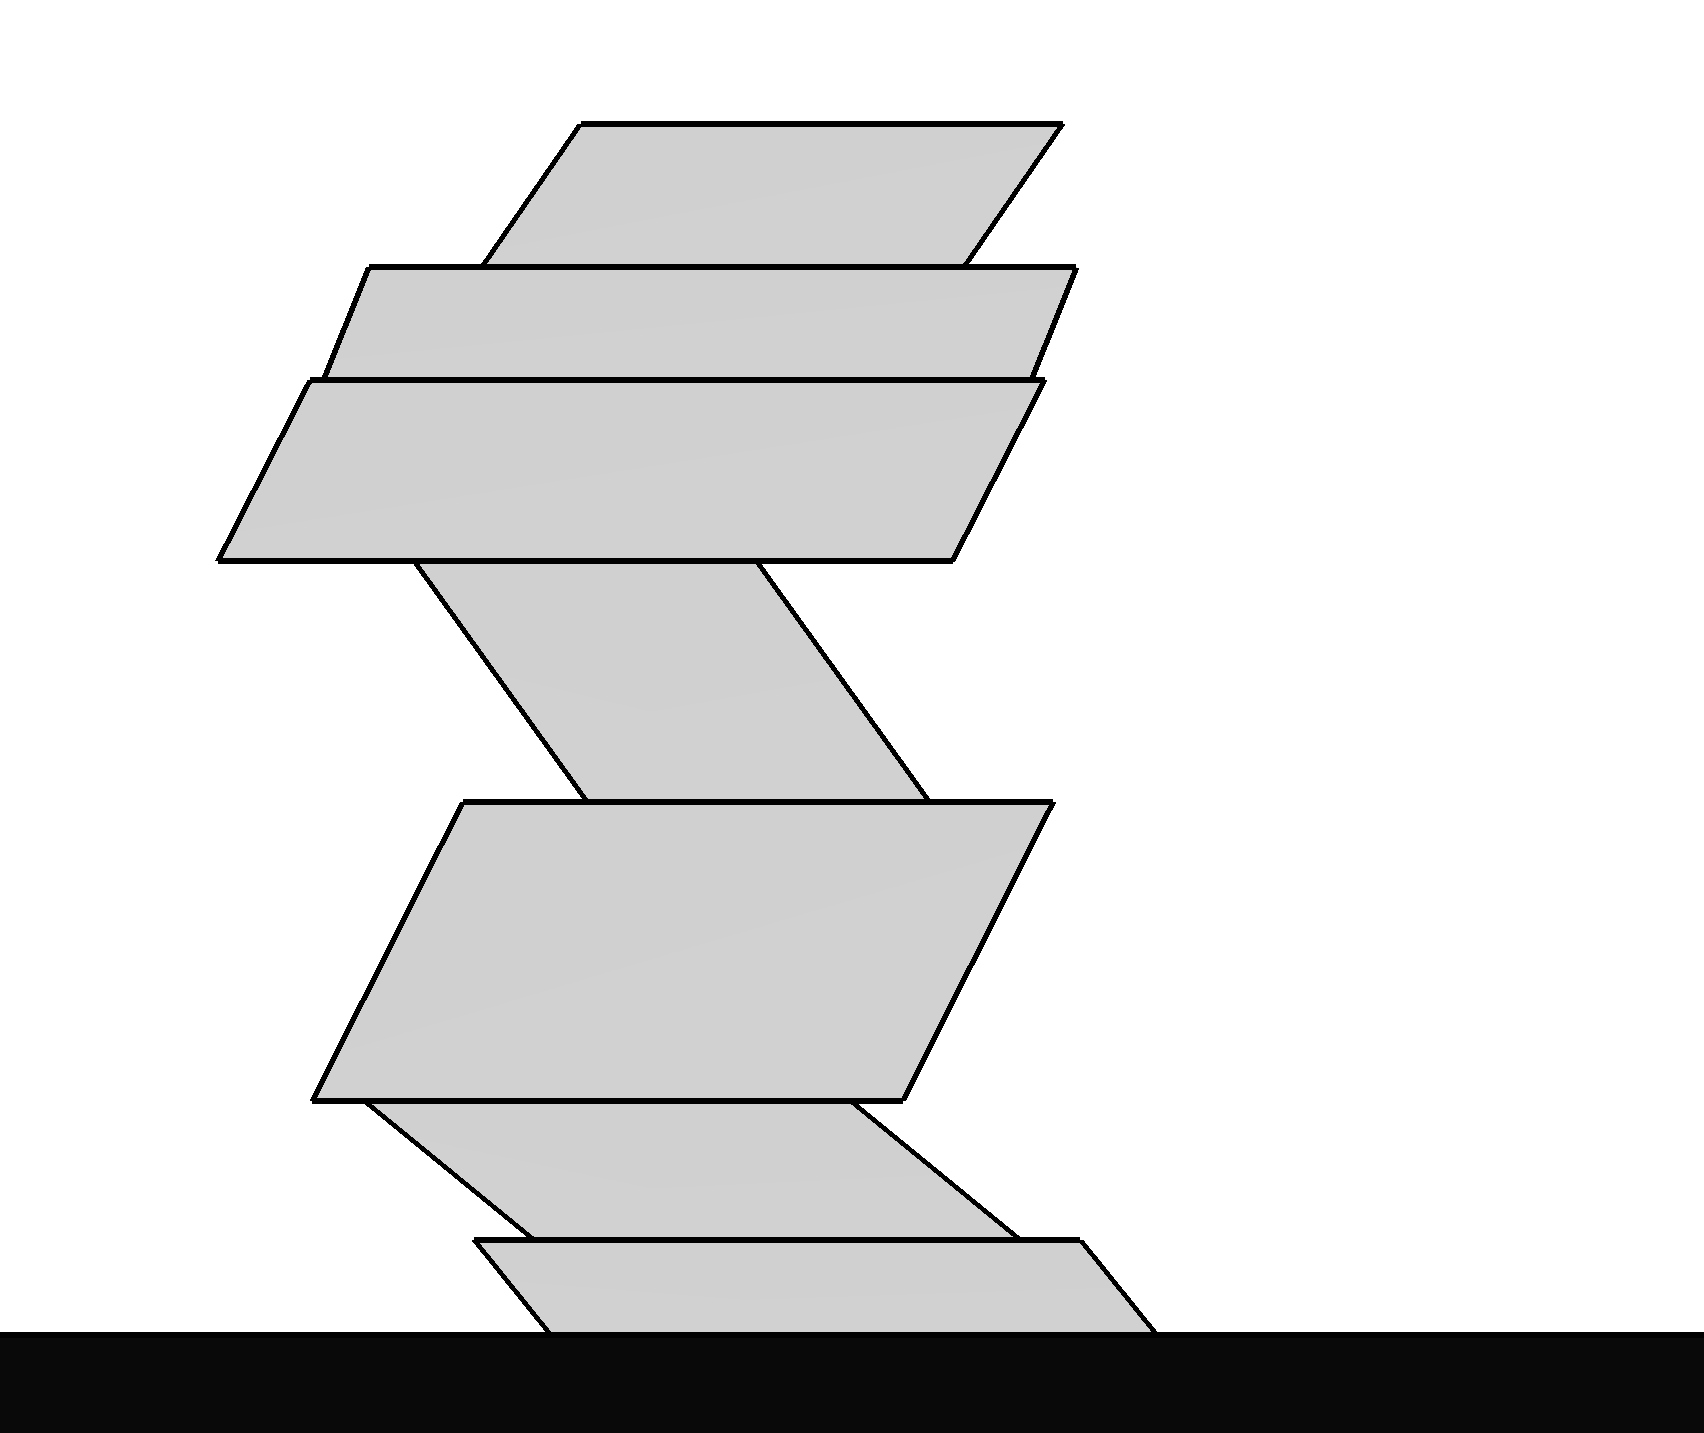
\includegraphics [trim={0.0cm 0.0cm 0cm 0.0cm},clip,width=1\textwidth]{\FigPath/tower2d}
				\caption{2D Planar Representation}
				\label{fig:t_2d}
			\end{subfigure}
			%
			\caption{Modelling Discrete Assemblies in Rhino}
			\label{fig:towers}
		\end{figure} 
	
		The following section will describe the workflow that was used to create, analyze, and label these assemblies in preparation for their use in an ML algorithm. 
	
		\subsection{Creating Geometry}
		
		Currently the dataset consists of towers assembled from of either uniform rectangular  or random  trapezoidal blocks joined at strictly horizontal planes (\Cref{fig:tower_types}). This horizontal joining is only chosen for simplicity, to ensure that there is no shear force at the interfaces - stability can therefore be determined purely on whether there exists any tensile forces at the interface. The foundation is modelled as a  solid black block, which extends infinitely in the frame of the image. The reasoning for representing this block as visually distinct from the rest of the tower this will be explained in more detail when discussing the ML algorithm.
		
		\newpage
		\begin{figure}[h]
			\centering
			%
			\begin{subfigure}[b]{0.49\textwidth}
				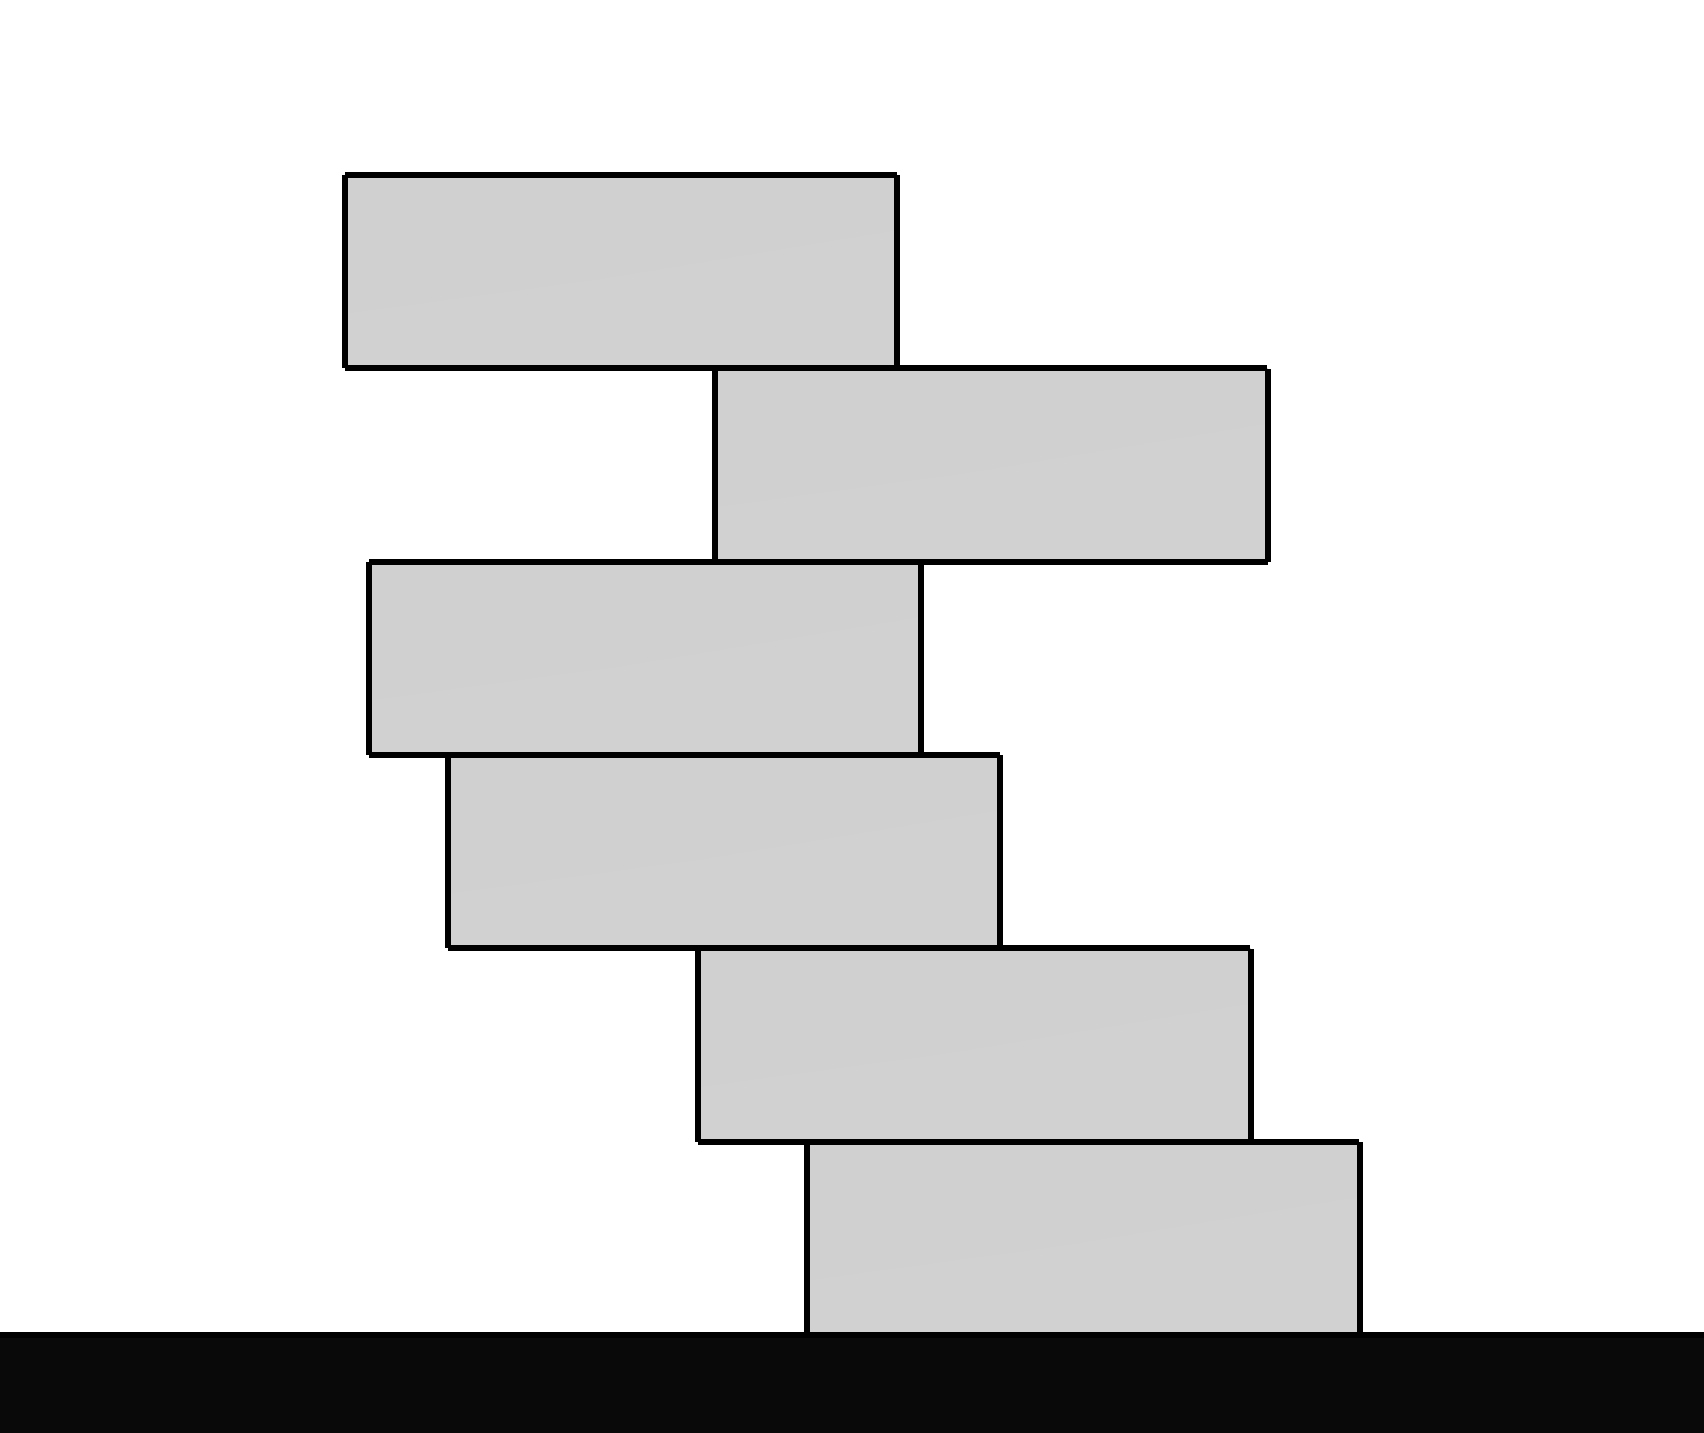
\includegraphics [trim={0.0cm 0cm 0cm 0.0cm},clip,width=1\textwidth]{\FigPath/tower_rect}
				\caption{Rectangular Blocks}
				\label{fig:t_}
			\end{subfigure}
			%
			\begin{subfigure}[b]{0.49\textwidth}
				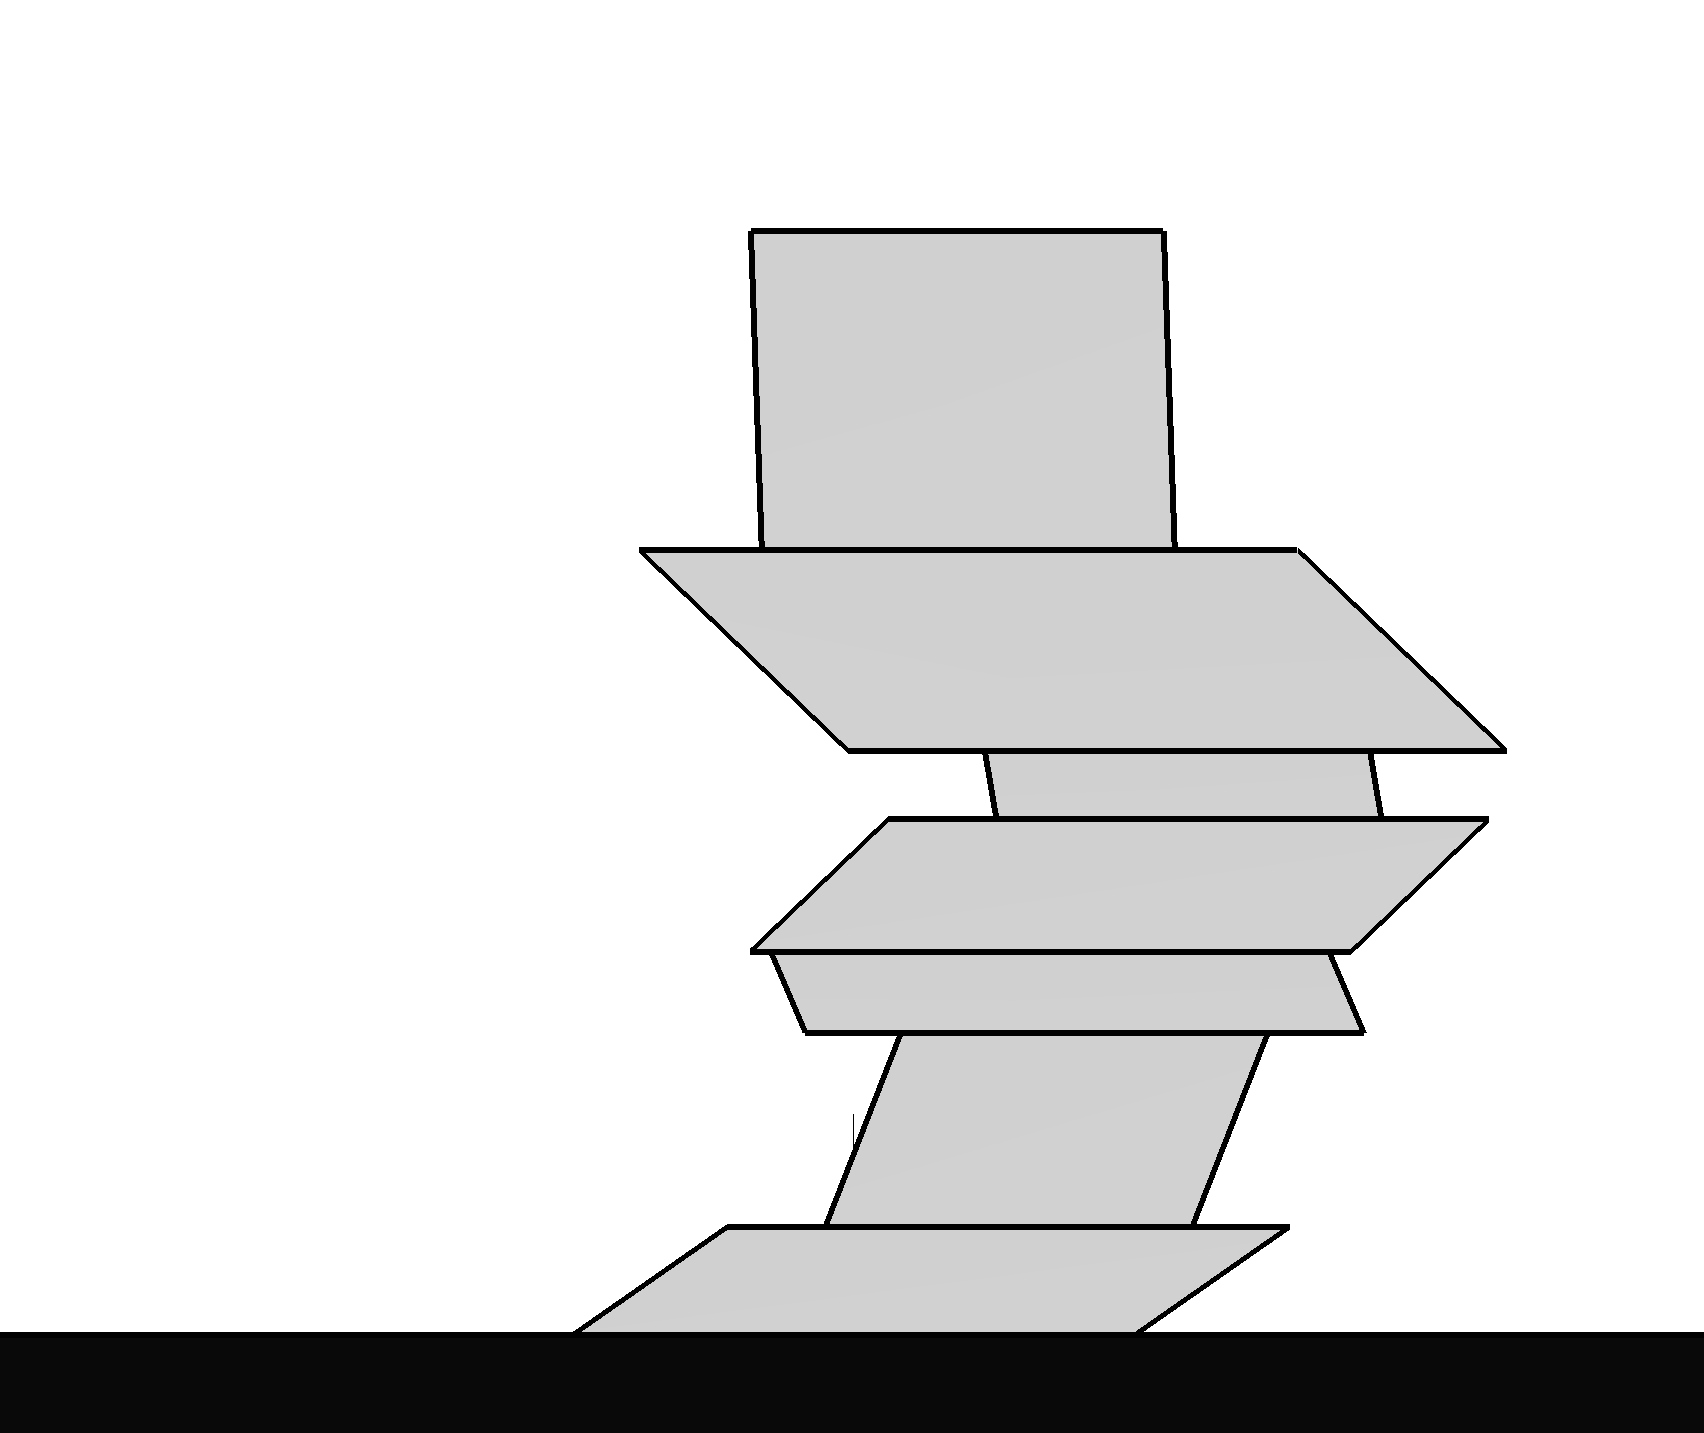
\includegraphics [trim={0.0cm 0.0cm 0cm 0.0cm},clip,width=1\textwidth]{\FigPath/tower_trap}
				\caption{Trapezoidal Blocks}
				\label{fig:t_trap}
			\end{subfigure}
			%
			\caption{Types of Towers}
			\label{fig:tower_types}
		\end{figure} 

		The geometry for a uniform rectangular tower is generated with the following process:
		\begin{enumerate}
			\item User specifies width, height, and depth for a block
			\item The block template is created as a closed Boundary Representation (Brep)
			\item User specifies number of blocks and a random seed
			\item Block is replicated vertically and shifted Left/Right by a random value
		\end{enumerate}
	
		The random seed method is a simple way to automate the creation of a random but replicable structure with just a single variable. The seed controls all the random shift values that are generated during the creation of one tower. By iterating through a list of seeds, a new tower is created each time the seed changes as all the blocks are assigned new random shifts.
		
		The trapezoidal tower is significantly more difficult to create as each block in the tower is unique. A randomly sized bottom plane is specified as the start of each new block (sitting on the top of the previous block), which is then extruded upwards by a random magnitude and direction resulting in a trapezoid. The random seed method is used again to ensure reproducibility of a random structure by just varying a single variable. In this case the seed controls variables such as the size of the base plane, the height of the block, direction of skew.
		
		Preliminary work has begun on generalizing the geometry generation further to blocks with inclined interfaces (\Cref{fig:tower_gen}). But at the current stage, not a large enough number of these towers were generated and analyzed to adequately influence the training of the NN (less than 10 \% of the whole dataset) - these inclined towers are therefore omitted from the analysis results that will be discussed in this paper.
		
		\begin{figure}[h]
			\centering
			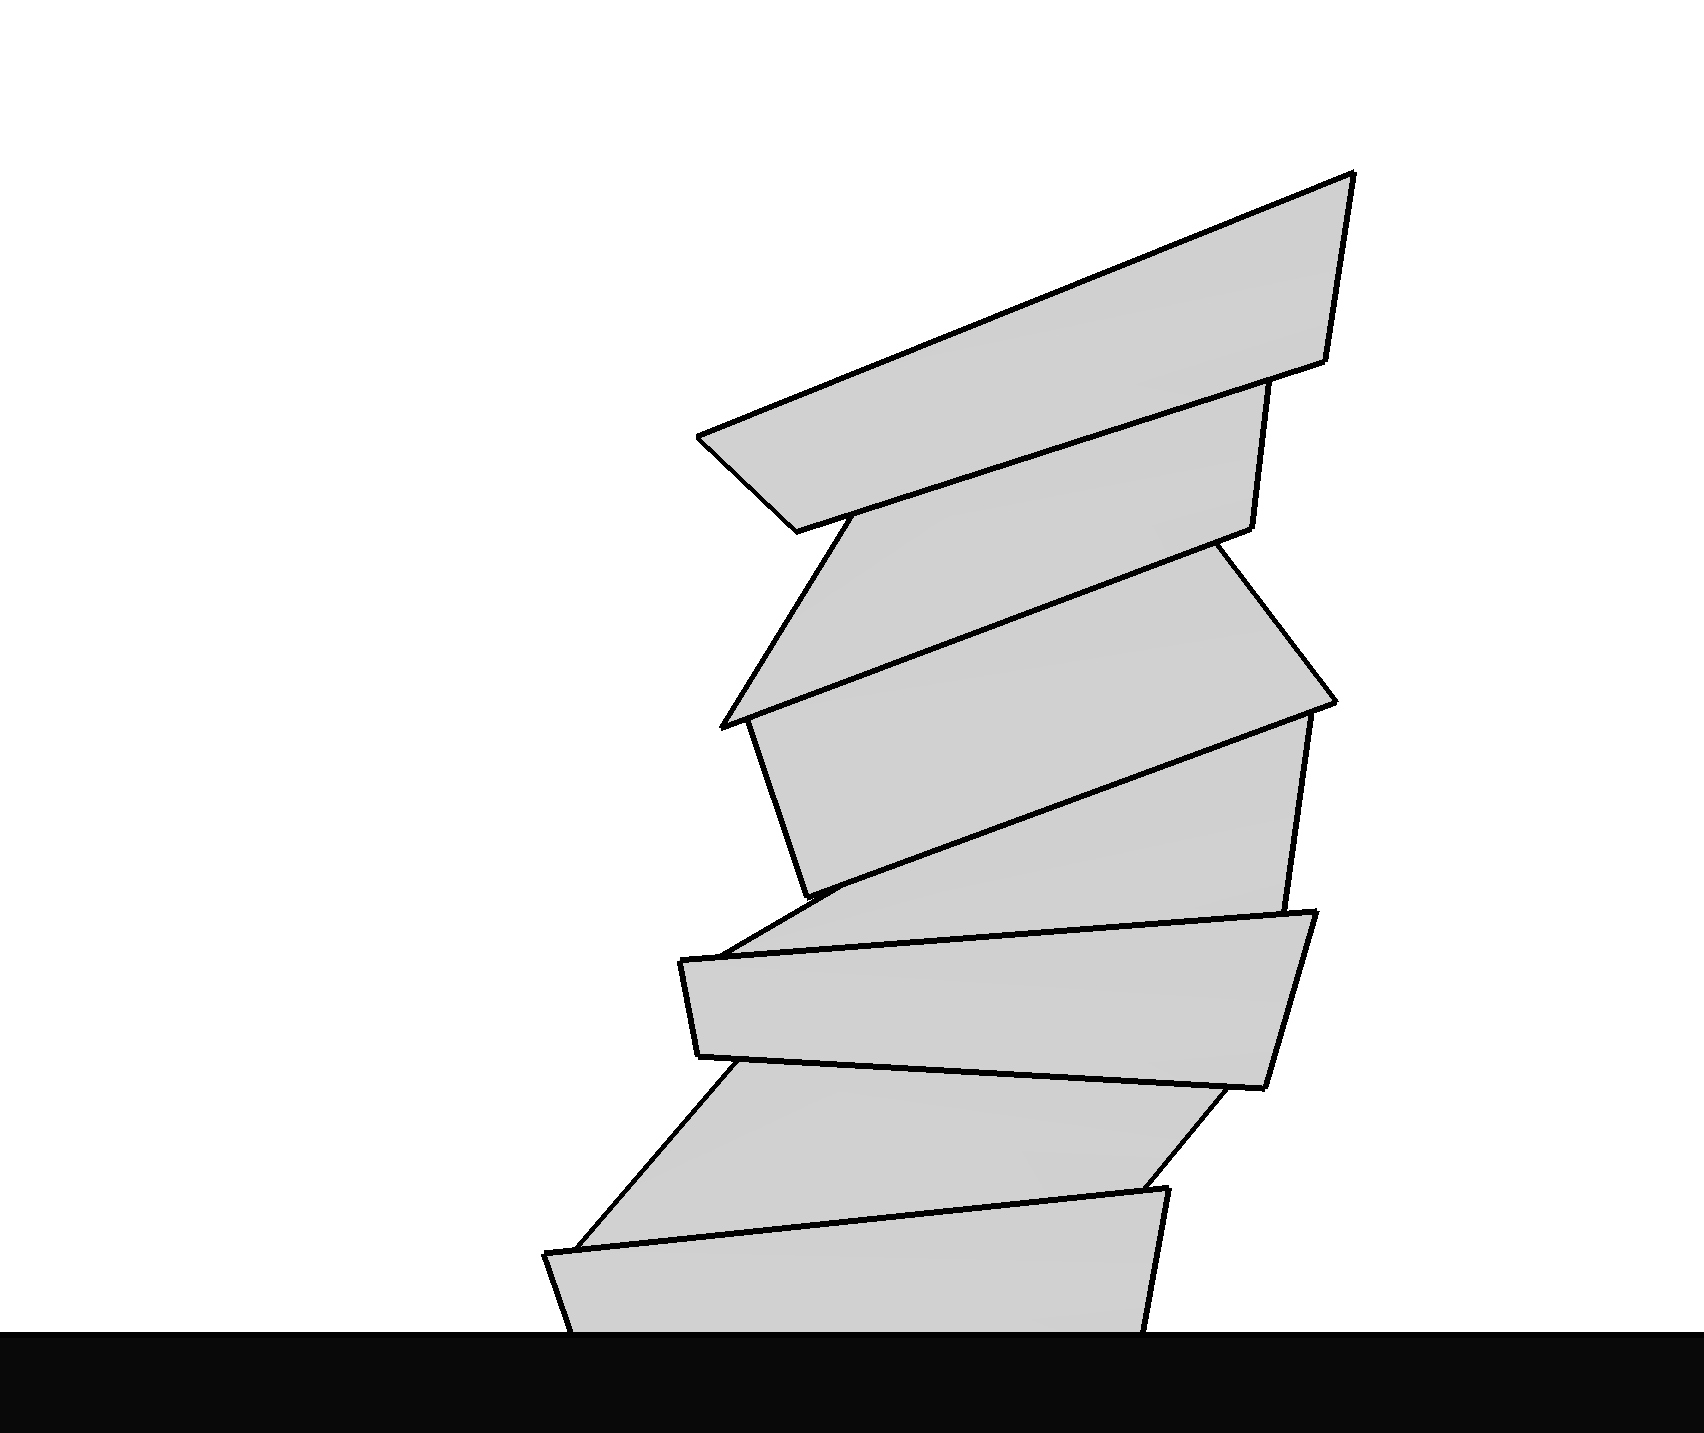
\includegraphics [trim={0.0cm 0cm 0cm 0.0cm},clip,width=0.7\textwidth]{\FigPath/tower_general}
			\caption{Tower with Inclined Inetrface Planes}
			\label{fig:tower_gen}
		\end{figure}
		
		\subsection{Analyzing Geometry}
		
			Talk about COMPAS Assembly and RBE		
			
		\subsection{Sorting Data}
	
	\newpage
	\section{Creating the Neural Network}
	
		\subsection{Architecture}
		
		\subsection{Parameters}
		
	\newpage
	\section{Results}
		
		\subsection{Tuning Parameters}
		
		
		
	
	
	\newpage
	%%%%%%%%%%%%%%%%%%%%%%%%%%%%
	\bibliographystyle{apa-good}\it
	\bibliography{stability}
	
	
\end{document}

